\section{Theorie}
\label{sec:Theorie}

\subsection{Aufbau und Funktionsweise einer Kathodenstrahlröhre}
\label{sec:kröhre}
Die Kathodenstrahlröhre besteht aus drei Elementen, welche sich in einer evakuierten Röhre befinden: Einer "Elektronenkanone", einem Ablenksystem und einem Leuchtschirm.
Dies ist schematisch in Abbildung \ref{fig:kröhre} dargestellt.
\begin{figure}
  \centering
  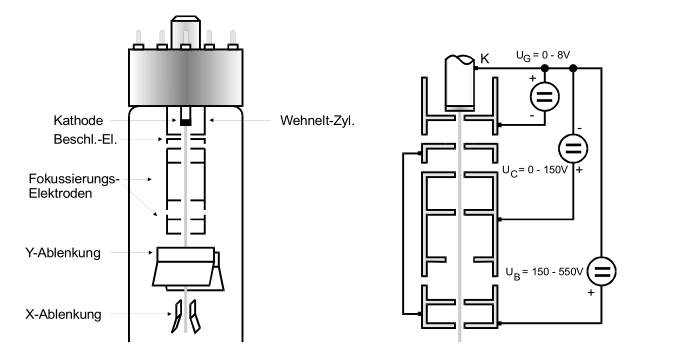
\includegraphics{images/kroehre.png}
  \caption{Schematischer Aufbau einer Kathodenstrahlröhre \cite{501}.}
  \label{fig:kröhre}
\end{figure}
In der "Elektronenkanone" werden durch Erhitzen einer Kathode, welche ein Zylinder aus einem Material mit einer niedrigen Elektronenaustrittsarbeit ist, Elektronen
freigesetzt. Dabei ist zu beachten, dass die Kathode indirekt durch einen Heizdraht erhitzt wird. Der die Kathode umgebende Wehnelt-Zylinder ist ein Hohlkörper mit
einer Bohrung in Strahlrichtung besitzt und an welchem ein negatives Potenzial, zur Steuerung der Intensität des Elektronenstrahls, anliegt.
Direkt im Anschluss liegt ein positives Potenzial an, welches die Elektronen beschleunigt. Quantitativ lässt sich die Geschwindigkeit entlang der Strahlrichtung als
\begin{equation}
  v_z = \sqrt{\frac{2 \, e_0 U_B}{m_0}}
  \label{eqn:vz}
\end{equation}
mit der Elektronenmasse $m_0$ und der Elementarladung $e_0$, beschreiben.
Durch eine sogennante Elektronenlinse, welche aus mehreren inhomogenen elektrischen Feldern besteht, wird der Elektronenstrahl weiter fokussiert.
Dann passiert er das Ablenksystem, welches aus zwei orthogonal zueinander ausgerichteten Kondensatoren besteht, und so die Elektronen ablenkt. Dies wird
im folgenden Kapitel beschrieben. Am Ende treffen die Elektronen auf einen Leuchtschirm, welcher bei Elektronenabsorption Photonen emittiert, und so den
Auftreffpunkt des Strahls sichtbar macht.

\subsection{Ablenkung von Elektronen im elektrischen Feld}
\label{sec:efeld}
Bewegen sich Elektronen mit einer konstanten Geschwindigkeit $v_z$ durch ein orthogonal zur Bewegungsrichtung verlaufendes homogenes elektrisches Feld, so werden
sie durch die Coulomb-Kraft abgelenkt. Wird das homogene Feld durch einen Kondensator mit der Spannung $U_d$, dem Plattenabstand $d$ und der Länge
$p$ erzeugt, ergibt sich für die Geschwindigkeit in die Ablenkungsrichtung $y$ der Elektronen folgender Ausdruck:
\begin{equation}
  v_y = \frac{e_0}{m_0} \frac{U_d}{d} \frac{p}{v_z}.
  \label{eqn:vy}
\end{equation}
Da sich die Elektronen in einer Kathodenstrahlröhre, welche in \ref{sec:kröhre} beschrieben wird, befinden, wird nun die Ablenkung der Elektronen von
dem Fall $U_d = 0$, welche auf dem Leuchtschirm der Kathodenstrahlröhre sichtbar ist, berechnet.
Der schematische Aufbau für welchen die Ablenkung berechnet werden soll ist in Abbildung \ref{fig:efeld} zu sehen.
\begin{figure}
  \centering
  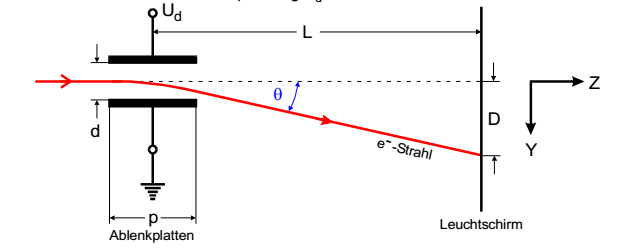
\includegraphics{images/efeld.png}
  \caption{Schematischer Aufbau der Ablenkung im elektrischen Feld \cite{501}.}
  \label{fig:efeld}
\end{figure}
Aus dem Winkel $\Theta = \sfrac{v_y}{v_z}$, und den Gleichungen \eqref{eqn:vy} und \eqref{eqn:vz} lässt sich
für die Ablenkung $D$ folgende Gleichung herleiten:
\begin{equation}
  D = \Theta \, L =  \frac{p}{2d} L \frac{U_d}{U_B}.
  \label{eqn:AblenkungEFeld}
\end{equation}
Dabei ist $L$ die Länge, welche der Elektronenstrahl nach der Ablenkung bis zum Leuchtschirm noch zurücklegen muss.
Wird keine konstante Ablenkspannung $U_d$ angelegt, sondern eine Wechselspannung, zum Beispiel in Form einer Sinusspannung, kann die Kathodenstrahlröhre auch
als Oszillograph fungieren. Dafür wird eine Sägezahnspannung als x-Ablenkung und die zu Untersuchende Wechselspannung als y-Ablenkung angelegt. Die Sägezahnspannung
dient dabei zur Erstellung einer x-Achse, gegen welche die zu untersuchende Spannung läuft. Dabei muss für ein stehendes Bild der zu Untersuchenden Spannung folgendes gelten:
\begin{equation}
  n \, {\nu}_\text{Sägezahn} = m \, {\nu}_\text{Untersuchung} \: \: \text{mit} \: n,m \in \symbb{N} \backslash \{0\} .
  \label{eqn:Oszillograph}
\end{equation}
Das bedeutet, dass die Frequenz der Sägezahnspannung ein rationales Vielfaches der Frequenz der zu Untersuchenden Spannung sein muss.

\subsection{Ablenkung von Elektronen im magnetischen Feld}
\label{sec:bfeld}
Wird die Kathodenstrahlröhre in ein magnetsiches Feld $\vec{B}$ gebracht, wirkt auf die Elektronen die Lorentz-Kraft
\begin{equation}
  \vec{F_L} =  q \, \vec{v} \times \vec{B}
  \label{eqn:Lorentz}
\end{equation}
welche nur von null verschieden ist, wenn die Geschwindigkeit $\vec{v}$ nicht parallel zum magnetischen Feld $\vec{B}$ ist.
Die Lorentz-Kraft ändert dabei nur die Richtung der Elektronen, jedoch nicht ihre Geschwindigkeit und damit auch nicht ihre kinetische Energie.
Die Ablenkung zwingt die Elektronen dabei auf eine Kreisbahn, deren Radius durch Gleichsetzen von Lorentz-Kraft und Zentrifugal-Kraft bestimmbar ist.
\begin{figure}
  \centering
  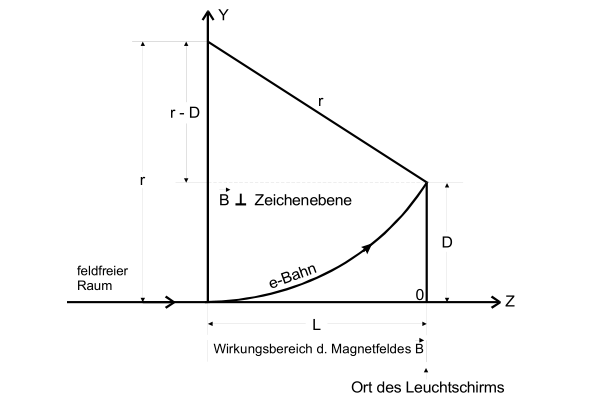
\includegraphics{images/bfeld.png}
  \caption{Schematischer Aufbau der Ablenkung im magnetischen Feld \cite{502}.}
  \label{fig:bfeld}
\end{figure}
Da der Radius aber schwer zu Messen ist, wird mittels der Beziehungen aus Abbildung \ref{fig:bfeld} und Gleichung \eqref{eqn:vz} folgender Ausdruck für die durch ein homogenes magnetisches Feld verursachte
Ablenkung des Elektronenstrahls auf dem Leuchtschirm der Kathodenstrahlröhre hergeleitet:
\begin{equation}
  \frac{D}{L^2 + D^2} = \frac{1}{\sqrt{8 U_B}} \sqrt{\frac{e_0}{m_0}} B .
  \label{eqn:AblenkungBFeld}
\end{equation}
Das homogene Feld wird dabei von einem Helmholtz-Spulenpaar erzeugt, bei welchem der Abstand der Spulen dem Radius der Spulen entspricht.
Für den Betrag der Feldstärke in der Mitte des Spulenpaares gilt
\begin{equation}
  B = {\mu}_0 \frac{8}{\sqrt{125}} \frac{N \, I}{R} .
  \label{eqn:hemlholtz}
\end{equation}
Dabei ist ${\mu}_0$ die magnetische Feldkonstante, $N$ die Windungszahl, und $I$ der angelegte Strom.
